\documentclass[11pt]{amsart}          
\usepackage[a4paper,verbose]{geometry}
\geometry{top=3cm,bottom=3cm,left=3cm,right=3cm,textheight=595pt}
\setlength{\parskip}{0.3em}
% ==============================
% PACKAGES
% ==============================

\usepackage{amsfonts}
\usepackage{amssymb}  
\usepackage{amsthm} 
\usepackage{amsmath} 
\usepackage{caption}
\usepackage[inline]{enumitem}
\setlist{itemsep=0em, topsep=0em, parsep=0em}
\setlist[enumerate]{label=(\alph*)}
\usepackage{etoolbox}
\usepackage{stmaryrd} 
\usepackage[dvipsnames]{xcolor}
\usepackage[]{hyperref}
\hypersetup{
  colorlinks,
  linkcolor=blue,
  citecolor=blue,
  urlcolor=blue}
\usepackage{graphicx}
\graphicspath{{assets/}}
\usepackage{mathtools}

\usepackage{tikz-cd}
\usepackage{minted}
\usepackage{float}
\usetikzlibrary{
  matrix,
  arrows,
  shapes
}

\setcounter{tocdepth}{1} % Sets depth for table of contents. 

\newcommand{\rr}{{\mathbb{R}}}
\newcommand{\nn}{{\mathbb{N}}}
\newcommand{\iso}{\cong}
\newcommand{\too}{\longrightarrow}
\newcommand{\tto}{\rightrightarrows}
\newcommand{\To}[1]{\xrightarrow{#1}}
\newcommand{\Too}[1]{\To{\;\;#1\;\;}}
\newcommand{\from}{\leftarrow}
\newcommand{\From}[1]{\xleftarrow{#1}}
\newcommand{\Cat}[1]{\mathbf{#1}}
\newcommand{\cat}[1]{\mathcal{#1}}
\newtheorem*{remark}{Remark}
\renewcommand{\ss}{\subseteq}
\newcommand{\hask}[1]{\mintinline{Haskell}{#1}}
\newenvironment{haskell}
  {\VerbatimEnvironment
  	\begin{minted}[escapeinside=??, mathescape=true,frame=single, framesep=5pt, tabsize=1]{Haskell}}
  {\end{minted}}

\author{Bartosz Milewski}
\title{Adjoint Functor Theorem}

\begin{document}
\maketitle{}

One of the tropes of detective movies is the almost miraculous ability to reconstruct an image from a blurry photograph. You just scan the picture,  say "enhance!", and voila, the face of the suspect or the registration number of their car appear on your computer screen. 

\begin{figure}[h]

\includegraphics{BladeRunner.jpeg}
\caption{Computer, enhance!}
\end{figure}

With constant improvements in deep learning, we might eventually be getting there. In category theory, though, we do this all the time. We recover lost information. The procedure is based on the basic tenet of category theory: an object is defined by its interactions with the rest of the world. This is the basis of all universal constructions, the Yoneda lemma, Grothendieck fibration, Kan extensions, and practically everything else. 

An iconic example is the construction of the left adjoint to a given functor, and that's what we are going to study here. But first let me explain why I decided to pick this subject, and how it's related to programming. I wanted to write a blog post about CPS (continuation passing style) and defunctionalization, and I stumbled upon an article in \href{https://ncatlab.org/nlab/show/defunctionalization}{nLab} that related defunctionalization to Freyd's Adjoint Functor Theorem; in particular to the Solution Set Condition. I had to figure this thing out.

Consider a functor $R$ from some category $\mathcal D$ to another category $\mathcal C$. 
\[R \colon D \to C \]
A functor, in general, loses some data, so it's normally impossible to invert it. It produces a "blurry" image of $\mathcal D$ inside $\mathcal C$. Its left adjoint is a functor from $\mathcal C$ to $\mathcal D$ 
\[ L \colon C \to D\]
that attempts to reconstruct lost information, to the best of its ability. Often the functor $R$ is \emph{forgetful}, which usually means that it purposefully forgets some information. Its left adjoint is then called \emph{free}, because it freely ad-libs the forgotten information. 


Of course it's not always possible, but under certain conditions such left adjoint exists. These conditions are spelled out in the Freyd General Adjoint Functor Theorem. 

To understand them, we have to talk a little about size issues. A lot of interesting categories are large. It means that there are so many objects in the category that they don't even form a set. The category of all sets, for instance, is large (there is no set of all sets). It's also possible that morphisms between two objects don't form a set. 

A category in which objects form a set is called \emph{small}, and a category in which hom-sets are sets is called \emph{locally small}. 

A lot of complexities in Freyd's theorem are related to size issues, so it's important to precisely spell out all the assumptions.

We assume that the source of the functor $R$, the category $\mathcal D$, is locally small. It must also be small-complete, that is, every small diagram in $\mathcal D$ must have a limit. (A small diagram is a functor from a small category.) We also want the functor $R$ to be continuous, that is, preserve all small limits. 

If it weren't for size issues, this would be enough to guarantee the existence of the left adjoint, and we'll first sketch the proof for this simplified case. In the general case, there is one more condition, the Solution Set Condition, which we'll discuss later.

Here's the problem we are trying to solve. We have the functor $R$ that maps objects and morphisms from $\mathcal D$ to $\mathcal C$. We want to define another functor $L$ that goes in the opposite direction. We're not looking for the inverse, so we're not expecting the composition of this functor with $R$ to be identity, but we want it to be \emph{related} to identity by two natural transformations called unit and counit. Their components are, respectively:
\[ \eta_c : c \to R L c\]
\[\epsilon_d : L R d \to d \]
and, as long as they satisfy some additional triangle identities, they will establish the adjunction $L \dashv R$.

We are going to define $L$ point-wise, so let's pick an object $c$ in $\mathcal C$ and try to propagate it back to $\mathcal D$. To do that, we have to gather as much information about $c$ as possible. We will then propagate all this information back to $\mathcal D$ and find an object in $\mathcal D$ that "looks the same." Think of this as creating a hologram of $c$ and shipping it back to $\mathcal D$. 

All information about $c$ is encoded in morphisms so, in order to generate our hologram, we'll gather all morphisms that originate in $c$. These morphisms form a category called the \emph{coslice} category $c/C$. 

The objects in $c/C$ are pairs $(x, f \colon c \to x)$. In other words, these are all the arrows that emanate from $c$, indexed by their target objects $x$. But what really defines the structure of this category are morphisms between these arrows. A morphism in $c/C$ from $(x, f)$ to $(y, g)$ is a morphism $h \colon x \to y$ that makes the following triangle commute:

\begin{figure}[H]
\centering
 \begin{tikzcd}
  & c
  \arrow[ld, "f"']
  \arrow[rd, "g"]\\
  x
  \arrow[rr, "h"]
  && y
\end{tikzcd}
\end{figure}

We now have complete information about $c$ encoded in the slice category, but we have no way to propagate it back to $\mathcal D$. This is because, in general, the image of $\mathcal D$ doesn't cover the whole of $\mathcal C$. Even more importantly, not all morphisms in $\mathcal C$ have corresponding morphisms in $\mathcal D$. We have to scale down our expectations, and define a partial hologram that does not capture all the information about $c$, but only this part which can be back-propagated to $\mathcal D$ using the functor $R$. Such partial hologram is called a comma category $c/R$.

The objects of $c/R$ are pairs $(d, f \colon c \to R d)$, where $d$ is an object in $\mathcal D$. In other words, these are all the arrows emanating from $c$ whose target is in the image of $R$. Again, the important structure is encoded in the morphisms of $c/R$. These are the arrows in $\mathcal D$, $h \colon d \to d'$ that make the following diagram commute in $\mathcal C$

\begin{figure}[H]
\centering
 \begin{tikzcd}
  & c
  \arrow[ld, "f"']
  \arrow[rd, "g"]\\
  R d
  \arrow[rr, "R h"]
  && R d'
\end{tikzcd}
\end{figure}
Notice an interesting fact: we can interpret these triangles as commutation conditions in a cone with a vertex $c$ and the base formed by a selection of objects and morphisms in the image of $R$. But not all objects or morphism in the image of $R$ are included. Only the morphisms that make the triangle commute--but these are exactly the morphisms that satisfy the cone condition. 

\begin{figure}[H]
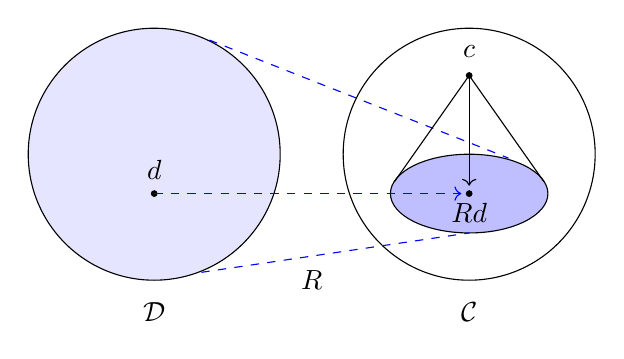
\begin{tikzpicture}
  \def\Xa{-2.0};
  \def\Xb{2.0};
  \def\Ytip{1.0};
  \def\Yo{-0.5};
  \def\Yb{-2.0};
         \draw (\Xa, 0)[fill=blue!10!white]  ellipse (1.6 and 1.6);
         \draw (\Xb , 0) ellipse (1.6 and 1.6);
         \draw (\Xb , \Yo)[fill=blue!25!white] ellipse (1 and 0.5);
         
        \filldraw (\Xb, \Ytip) circle (1pt);
        \node at ( \Xb, \Ytip + 0.3) { $c$ };
        
        \filldraw (\Xa, \Yo) circle (1pt);
        \node at ( \Xa, \Yo + 0.3) { $d$ };
        
        \filldraw (\Xb, \Yo) circle (1pt);
        \node at ( \Xb, \Yo - 0.25) { $R d$ };
	\draw[->, blue, dashed] (\Xa, \Yo) -- (\Xb - 0.1, \Yo);
	
	\draw[->] (\Xb, \Ytip) -- (\Xb, \Yo + 0.1);
        
        \node at (\Xa, \Yb) { $\mathcal D$ };
        \node at (\Xb, \Yb) { $\mathcal C$ };
        \node at (0, \Yb + 0.4) { $R$ };

	\draw [blue, dashed] (\Xa + 0.7, \Ytip + 0.45) -- (\Xb + 0.5, \Yo + 0.45);
	\draw [blue, dashed] (\Xa + 0.6, \Yo - 1) -- (\Xb, \Yo - 0.5);
	
	\draw (\Xb, \Ytip) -- (\Xb + 0.95, \Yo + 0.15);
	\draw (\Xb, \Ytip) -- (\Xb - 0.95, \Yo + 0.15);

\end{tikzpicture}
\end{figure}

We can now take all this information about $c$ that's been encoded in $c/R$ and move it back to $\mathcal D$. We define a projection functor $\pi_c \colon c/R \to D$ that maps $(d, f)$ to $d$, thus forgetting the morphism $f$. What's important, though, is that it keeps the information encoded in the morphisms of $c/R$, because these are just morphisms in $\mathcal D$.

\begin{figure}[H]
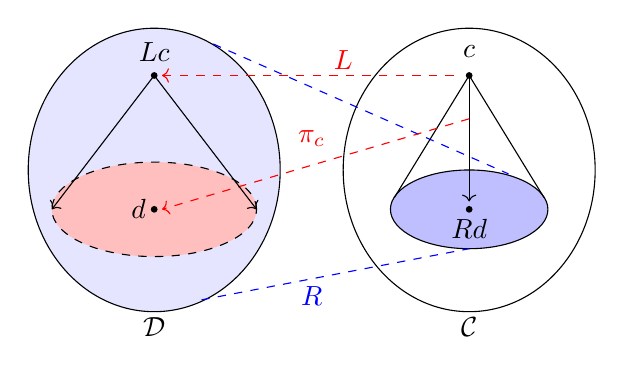
\begin{tikzpicture}
  \def\Xa{-2.0};
  \def\Xb{2.0};
  \def\Ytip{1.2};
  \def\Yo{-0.5};
  \def\Yb{-2.0};
         \draw (\Xa, 0)[fill=blue!10!white]  ellipse (1.6 and 1.8);  % D
         \node at (\Xa, \Yb) { $\mathcal D$ };
         \draw (\Xb , 0) ellipse (1.6 and 1.8);                               % C
         \node at (\Xb, \Yb) { $\mathcal C$ };
         \draw (\Xb , \Yo)[fill=blue!25!white] ellipse (1 and 0.5);  % R D
         \draw (\Xa , \Yo)[fill=red!25!white, dashed] ellipse (1.3 and 0.6); % pi c
         
	\draw [blue, dashed] (\Xa + 0.75, \Ytip + 0.40) -- (\Xb + 0.5, \Yo + 0.45);
	\draw [blue, dashed] (\Xa + 0.6, \Yo - 1.15) -- (\Xb, \Yo - 0.5);
        \node [blue] at (0, \Yb + 0.4)        { $R$ };
         
       \filldraw (\Xb, \Ytip) circle (1pt);
        \node at ( \Xb, \Ytip + 0.3)           { $c$ };
        
        \filldraw (\Xb, \Yo) circle (1pt);
        \node at ( \Xb, \Yo - 0.25)            { $R d$ };
	
	\draw[->] (\Xb, \Ytip) -- (\Xb, \Yo + 0.1);  % c -> Rd
	\draw (\Xb, \Ytip) -- (\Xb + 0.95, \Yo + 0.15);
	\draw (\Xb, \Ytip) -- (\Xb - 0.95, \Yo + 0.15);

        \draw[->, red, dashed] (\Xb, \Ytip - 0.55) -- (\Xa + 0.1 , \Yo);  % pi_c: (d, f) -> d
        \node [red] at (0, \Ytip - 0.8)       { $\pi_c$ };
        \node at (\Xa - 0.2 , \Yo)             { $d$ };
        \filldraw (\Xa, \Yo) circle (1pt);
	
	\draw[<-, red, dashed] (\Xa + 0.1, \Ytip) -- (\Xb - 0.1, \Ytip); % c -> L c
        \node [red] at (0.4, \Ytip + 0.2)  { $L$ };
        \filldraw (\Xa, \Ytip) circle (1pt);
        \node at (\Xa, \Ytip + 0.3)         { $L c$ };

        \draw[->] (\Xa, \Ytip) -- (\Xa - 1.3, \Yo);   % Lc -> pi
        \draw[->] (\Xa, \Ytip) -- (\Xa + 1.3, \Yo);  % Lc -> pi
        
\end{tikzpicture}
\end{figure}

The image of $\pi_c$ doesn't necessarily cover the whole of $\mathcal D$, because not every $R d$ has arrows coming from $c$. Similarly, only the morphisms that make the appropriate triangle in $\mathcal C$ commute are picked by $\pi_c$. But those objects and morphisms that \emph{are} in the image of $\pi_c$ form a diagram in $\mathcal C$. This diagram is our partial hologram, and we can use it to pick an object in $\mathcal D$ that looks almost exactly like $c$. That object is the limit of this diagram. We pick this object as the definition of $L c$: the left adjoint of $R$ acting on $c$.

Here's the tricky part: we assumed that $\mathcal D$ was small-complete, so every small diagram had a limit; but the diagram defined by $\pi_c$ is not necessarily small. Let's ignore this problem for a moment, and continue sketching the proof. We want to show that the mapping that assigns the limit of $\pi_c$ to every $c$ is left adjoint to $R$. 

Let's see if we can define the unit of the adjunction:
\[ \eta_c : c \to R L c\]
We have defined $L c$ as the limit of the diagram $\pi_c$. We also assumed that $R$ preserves limits (small limits, really; but we are ignoring size problems for the moment). It means that $R L c$ must be the limit of the diagram $R \pi_c$ in $\mathcal C$. But, as we noted before, the diagram  $R \pi_c$ is exactly the base of the cone with the apex $c$ that was used to define the comma category $c/R$. Since $R L c$ is the limit of this diagram, there must be a unique morphism from any other cone to it. In particular there is a morphism from $c$ to it, and that's the morphism we'll chose as our $\eta_c$. 

\begin{figure}[H]
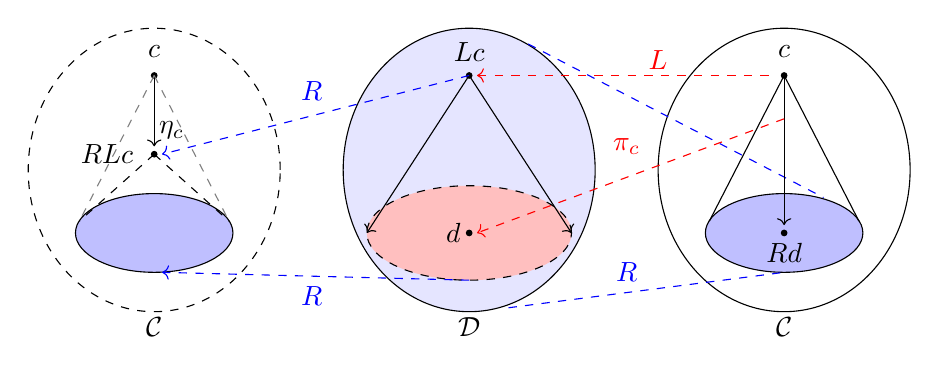
\begin{tikzpicture}
  \def\Xc{-4.0};
  \def\Xa{0.0};
  \def\Xb{4.0};
  \def\Ytip{1.2};
  \def\Yo{-0.8};
  \def\Yb{-2.0};
  \def\Ym{0.2};
         \draw (\Xc, 0) [dashed] ellipse (1.6 and 1.8);  % C
         \node at (\Xc, \Yb) { $\mathcal C$ };
         \draw (\Xa, 0)[fill=blue!10!white]  ellipse (1.6 and 1.8);  % D
         \node at (\Xa, \Yb) { $\mathcal D$ };
         \draw (\Xb , 0) ellipse (1.6 and 1.8);                               % C
         \node at (\Xb, \Yb) { $\mathcal C$ };
         \draw (\Xb , \Yo)[fill=blue!25!white] ellipse (1 and 0.5);  % R D
         \draw (\Xc , \Yo)[fill=blue!25!white] ellipse (1 and 0.5);  % R D
         \draw (\Xa , \Yo)[fill=red!25!white, dashed] ellipse (1.3 and 0.6); % pi c
         
	\draw [blue, dashed] (\Xa + 0.75, \Ytip + 0.40) -- (\Xb + 0.5, \Yo + 0.45);
	\draw [blue, dashed] (\Xa + 0.5, \Yo - 0.95) -- (\Xb, \Yo - 0.5);
        \node [blue] at (2, \Yb + 0.7)        { $R$ };
         
       \filldraw (\Xb, \Ytip) circle (1pt);
        \node at ( \Xb, \Ytip + 0.3)           { $c$ };
        
        \filldraw (\Xb, \Yo) circle (1pt);
        \node at ( \Xb, \Yo - 0.25)            { $R d$ };
	
	\draw[->] (\Xb, \Ytip) -- (\Xb, \Yo + 0.1);  % c -> Rd
	\draw (\Xb, \Ytip) -- (\Xb + 0.95, \Yo + 0.15);
	\draw (\Xb, \Ytip) -- (\Xb - 0.95, \Yo + 0.15);

        \draw[->, red, dashed] (\Xb, \Ytip - 0.55) -- (\Xa + 0.1 , \Yo);  % pi_c: (d, f) -> d
        \node [red] at (2.0, \Ytip - 0.9)       { $\pi_c$ };
        \node at (\Xa - 0.2 , \Yo)             { $d$ };
        \filldraw (\Xa, \Yo) circle (1pt);
	
	\draw[<-, red, dashed] (\Xa + 0.1, \Ytip) -- (\Xb - 0.1, \Ytip); % c -> L c
        \node [red] at (2.4, \Ytip + 0.2)  { $L$ };
        \filldraw (\Xa, \Ytip) circle (1pt);
        \node at (\Xa, \Ytip + 0.3)         { $L c$ };

        \draw[->] (\Xa, \Ytip) -- (\Xa - 1.3, \Yo);   % Lc -> pi
        \draw[->] (\Xa, \Ytip) -- (\Xa + 1.3, \Yo);  % Lc -> pi
        
        \draw[->, blue, dashed] (\Xa, \Ytip) -- (\Xc + 0.1, \Ym);   % Lc -> RLc
        \node [blue] at ( \Xc * 0.5 + \Xa * 0.5, \Ym + 0.8)            { $R$ };
        
       \filldraw (\Xc, \Ytip) circle (1pt);
        \node at ( \Xc, \Ytip + 0.3)           { $c$ };
        
        \filldraw (\Xc, \Ym) circle (1pt);
        \node at ( \Xc - 0.6, \Ym)            { $RLc$ };
	
	\draw[->] (\Xc, \Ytip) -- (\Xc, \Ym + 0.1);  % eta
        \node at ( \Xc + 0.22, \Ym + 0.3)            { $\eta_c$ };
	\draw [dashed, gray] (\Xc, \Ytip) -- (\Xc + 0.95, \Yo + 0.15);
	\draw [dashed, gray] (\Xc, \Ytip) -- (\Xc - 0.95, \Yo + 0.15);
	\draw [dashed] (\Xc,  \Ym) -- (\Xc + 0.95, \Yo + 0.15);
	\draw [dashed] (\Xc,  \Ym) -- (\Xc - 0.95, \Yo + 0.15);

        \draw[->, blue, dashed] (\Xa, \Yo - 0.6) -- (\Xc + 0.1, \Yo - 0.5);   % diagrams
        \node [blue] at ( \Xc * 0.5 + \Xa * 0.5, \Yo - 0.8)            { $R$ };

\end{tikzpicture}
\end{figure}



Incidentally, we can also interpret $\eta_c$ as an object of the comma category $c/R$, namely $(Lc, \eta_c \colon c \to R L c)$. In fact, this is the \emph{initial object} in that category. If you pick any other object $(d, g \colon c \to R d)$, you can always find a morphism $h \colon L c \to d$, which is just a leg, a projection, in the limiting cone that defines $L c$. It is automatically a morphism in $c/R$ because the following triangle commutes:

\begin{figure}[H]
\centering
 \begin{tikzcd}
  c
  \arrow[d, "\eta_c"']
  \arrow[rdd, "g"] \\
  R L c
  \arrow[rd, "R h"'] \\
  & R d
\end{tikzcd}
\end{figure}
This is the triangle that defines $\eta_c$ as a morphism of cones, from the top cone with the apex $c$, to the bottom (limiting) cone with the apex $R L c$. It's possible to show that $h$ is a unique such morphism and, therefore, $\eta_c$ is initial in $c/R$. We'll use this interpretation later, when discussing the full version of the Freyd's theorem.

We can also define the counit of the adjunction. Its component at $c$ is a morphism
\[\epsilon_d : L R d \to d \]
First, we perform our construction starting with $c = R d$. We define the comma category $R d / R$ and use $\pi_{R d}$ to create the diagram whose limit is $L R d$. We pick $\epsilon_d$ to be a projection in the limiting cone. We are guaranteed that $d$ is in the base of the cone, because it's the image of $(d, id \colon R d \to R d)$ under $\pi_{R d}$. 

To complete this proof, one should show that the unit and counit are natural transformations and that they satisfy triangle identities. 

So what about those pesky size issues? It's one thing to demand the existence of all small limits, and a completely different thing to demand the existence of all large limits. Since the comma category may be too large, maybe we can cut it down to size by carefully picking up a (small) set of objects out of all objects of $\mathcal D$. We may take some indexing set $I$ and construct a family $d_i$ of objects of $\mathcal D$ indexed by elements of $I$. It doesn't have to be one family for all---we may pick a different family for every object $c$ for which we are performing our construction. 

Instead of using the whole comma category $c/R$, we'll limit ourselves to a set of arrows $f_i \colon c \to R d_i$. But in a comma category we also had morphisms between arrows. In fact they were the essential carriers of the structure of the comma category. Let's have another look at these morphisms.

\begin{figure}[H]
\centering
 \begin{tikzcd}
  & c
  \arrow[ld, "f"']
  \arrow[rd, "g"]\\
  R d
  \arrow[rr, "R h"]
  && R d'
\end{tikzcd}
\end{figure}

This commuting condition can be re-interpreted as describing a factorization of $g$ through $f$. It so happens that every morphism $g$ can be trivially factorized by  picking $d = d'$ and $h = id_d$. But if we restrict the factors $f$ to be members of the family $f_i$ then not every $g \colon c \to R d$  (for arbitrary $d$) can be automatically factorized. We have to demand it. We have the following:

\emph{Solution Set Condition}: For every object $c$ there exists a small set $I$ with an $I$-indexed family of objects $d_i$ in $\mathcal D$ and a family of morphisms $f_i \colon c \to R d_i$, such that every morphism $g \colon c \to R d$ can be factored through one of $f_i$. That is, there exists a morphism $h \colon d_i \to d$ such that
\[g = R h \circ f_i \]

\begin{figure}[H]
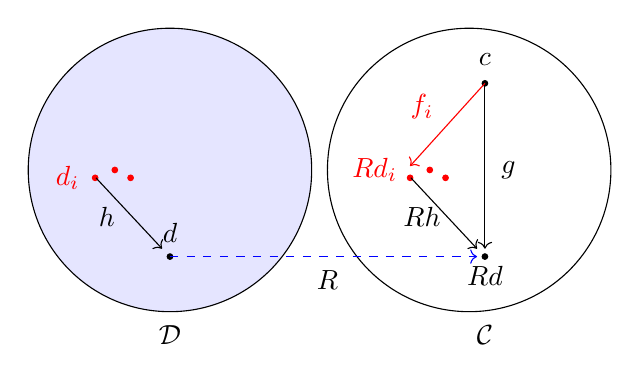
\begin{tikzpicture}
  \def\Xa{-2.0};
  \def\Xb{2.0};
  \def\Ytip{1.0};
  \def\Yo{-1.2};
  \def\Ym{-0.2};
  \def\Yb{-2.0};
         \draw (\Xa, -0.1)[fill=blue!10!white]  ellipse (1.8 and 1.8);
         \draw (\Xb - 0.2 , -0.1) ellipse (1.8 and 1.8);
         
        \filldraw (\Xb, \Ytip) circle (1pt);
        \node at ( \Xb, \Ytip + 0.3) { $c$ };
        
        \filldraw [red] (\Xa - 0.95, \Ym) circle (1pt);
        \filldraw [red] (\Xa - 0.70, \Ym + 0.1) circle (1pt);
        \filldraw [red] (\Xa - 0.50, \Ym) circle (1pt);
        \node [red] at (\Xa - 1.3, \Ym) { $d_i$ };
	\draw[->] (\Xa - 0.94, \Ym) -- (\Xa - 0.1, \Yo + 0.1);
        \filldraw (\Xa, \Yo) circle (1pt);
        \node at ( \Xa, \Yo + 0.3) { $d$ };
        \node at (\Xa - 0.8, \Ym - 0.5) { $h$ };
        
        \filldraw (\Xb, \Yo) circle (1pt);
        \node at ( \Xb, \Yo - 0.25) { $R d$ };
	\draw[->, blue, dashed] (\Xa, \Yo) -- (\Xb - 0.1, \Yo);
	
	\draw[->] (\Xb, \Ytip) -- (\Xb, \Yo + 0.1);
        
        \node at (\Xa, \Yb - 0.2) { $\mathcal D$ };
        \node at (\Xb, \Yb - 0.2) { $\mathcal C$ };
        \node at (0, \Yo - 0.3) { $R$ };

	
	\draw[->, red] (\Xb, \Ytip) -- (\Xb - 0.95, \Ym + 0.15);
        \filldraw [red] (\Xb - 0.95, \Ym) circle (1pt);
        \node [red] at (\Xb - 1.4, \Ym + 0.1) { $R d_i$ };
        \node [red] at (\Xb - 0.8, \Ym + 0.9) { $f_i$ };
        \filldraw [red] (\Xb - 0.70, \Ym + 0.1) circle (1pt);
        \filldraw [red] (\Xb - 0.50, \Ym) circle (1pt);
	\draw[->] (\Xb - 0.94, \Ym) -- (\Xb - 0.1, \Yo + 0.1);
        \node at (\Xb - 0.8, \Ym - 0.5) { $R h$ };
        \node at (\Xb + 0.3, \Ym + 0.1) { $g$ };

\end{tikzpicture}
\end{figure}

There is a shorthand for this statement: All comma categories $c/R$ admit weakly initial families of objects. We'll come back to it later.

We can now formulate:

\emph{Freyd's Adjoint Functor Theorem}: If $\mathcal D$ is a locally small and small-complete category, and the functor $R \colon D \to C$ is continuous (small-limit preserving), and it satisfies the solution set condition, then $R$ has a left adjoint.

We've seen before that the key to defining the point-wise left adjoint is to find the initial object in the comma category $c/R$. The problem is that this comma category may be large. So the trick is to split the proof into two parts: first defining a \emph{weakly} initial object, and then constructing the actual initial object using equalizers. A weakly initial object has morphisms to every object in the category but, unlike its strong version, these morphisms don't have to be unique. 

An even weaker notion is that of a weakly initial set of objects. These are objects that among themselves have arrows to every object in the category, but it's possible that no individual object has all the arrows. The solution set in Freyd's theorem is such a weakly initial set in the comma category $c/R$. Since we assumed that $\mathcal C$ is small-complete, we can take a product of these objects and show that it's weakly initial. The proof then proceeds with the construction of the initial object. 

The details of the proof can be found in any category theory text or in \href{https://ncatlab.org/nlab/show/adjoint+functor+theorem}{nLab}. 

Next we'll see the application of these results to the problem of defunctionalization of computer programs.

\end{document}


